\documentclass[border = 1.5cm]{standalone}
%\documentclass[border = 1.5cm, convert={density=300,size=1080x800,outext=.png}]{standalone} % doesn't work
%%%% packages
\usepackage{tikz}
\usetikzlibrary{trees, arrows, shapes.geometric, positioning} % TikZ libraries
%%%% layers
\pgfdeclarelayer{bg1}    % declare background layer
\pgfdeclarelayer{bg2}
\pgfdeclarelayer{bg3}
\pgfsetlayers{bg3,bg2,bg1,main}  % set the order of the layers (main is the standard layer)

%%%% styles
\tikzset{
	every rectangle node/.style = {thick, anchor=west},
	every picture/.style = {/utils/exec={\sffamily}},
	font = {\fontsize{13pt}{12}\selectfont},
	io/.style = {rectangle, minimum width = 4cm, minimum height = 3cm, text centered, draw = black, fill = blue!10},
	main/.style = {rectangle, draw = black, rounded corners, minimum width = 3cm, minimum height = 1.25cm, text centered},
	etox-base/.style = {rectangle, rounded corners},
	etox-base-shiny/.style = {circle},
	ids/.style = {diamond, minimum width = 3cm, minimum height = 2cm, text centered, draw = black, fill = green!30},
	res/.style = {rectangle, rounded corners, minimum width = 2cm, minimum height = 1cm, text centered, draw = black, fill = blue!30},
	resvariables/.style = {rectangle, minimum width = 2cm, minimum height = 1cm, text centered},
	steps/.style = {rectangle, minimum width = 1cm, text centered, fill = yellow},
	arrow/.style = {->, > = stealth, draw = black, color = gray!80, line width = 2.5pt}
}

\begin{document}
	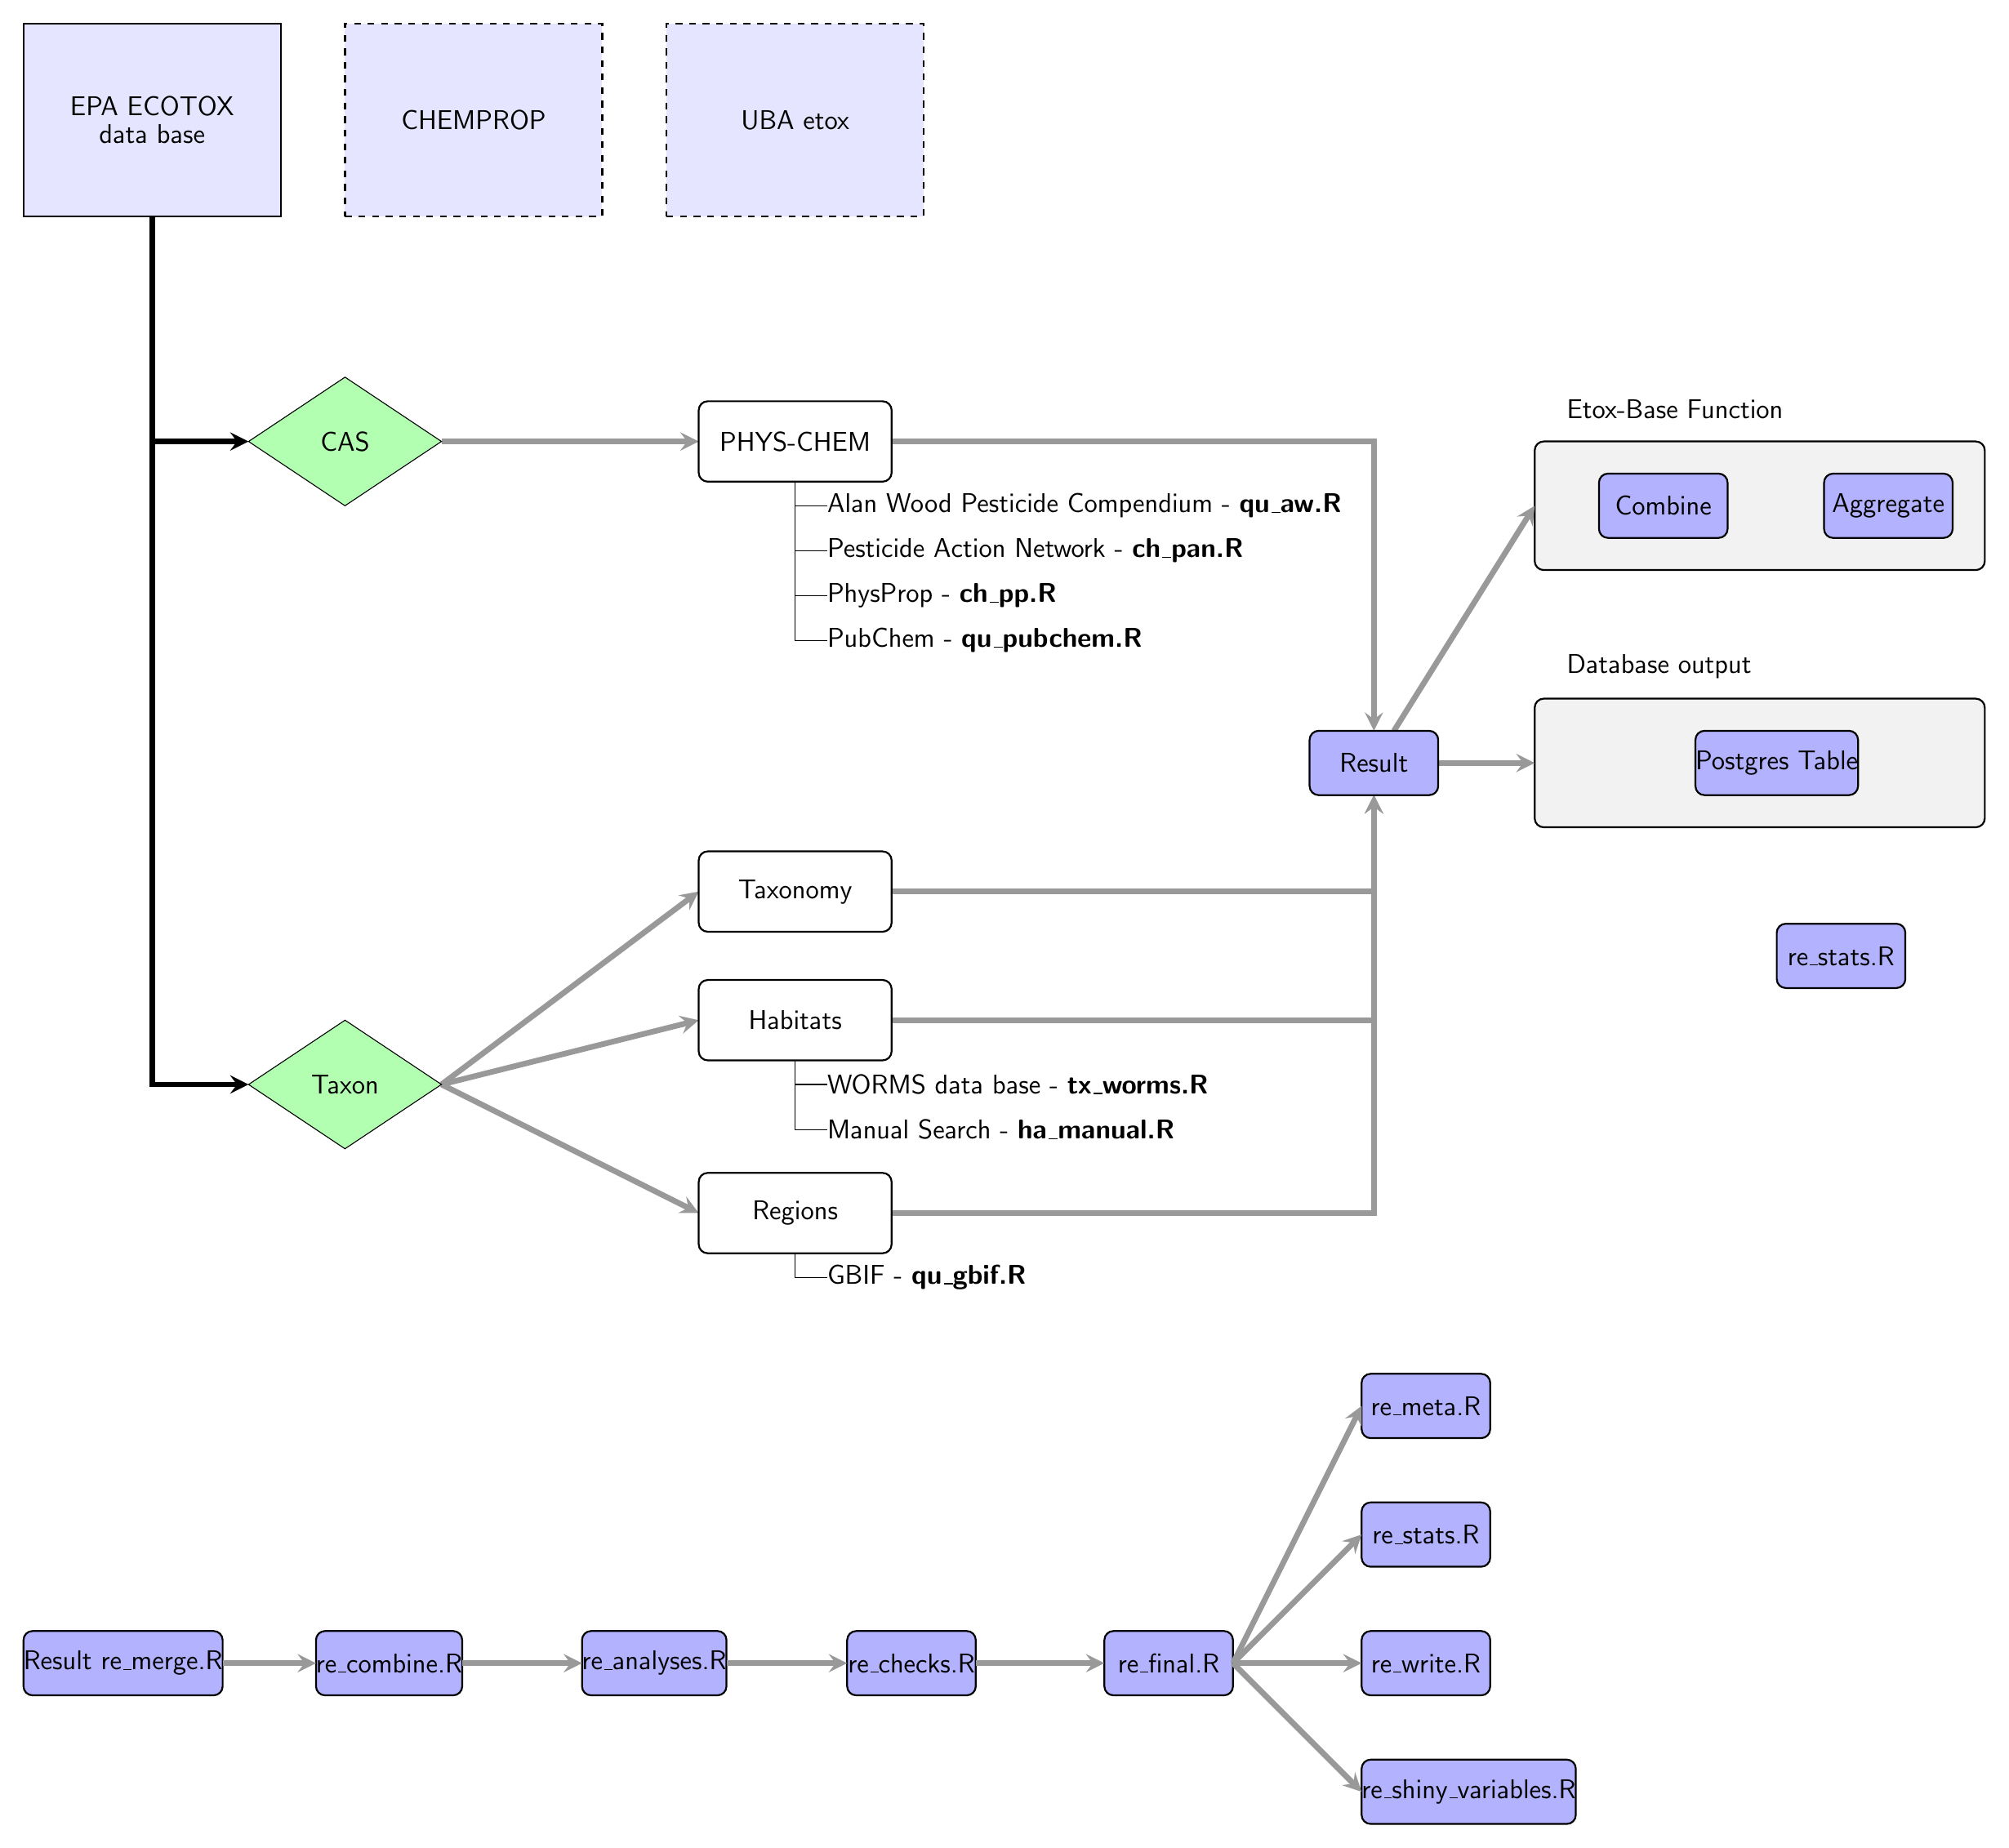
\begin{tikzpicture}[
	grow via three points={one child at (0.5,-1) and
		two children at (0.5,-1) and (0.5,-1.7)},
	edge from parent path={(\tikzparentnode.south) |- (\tikzchildnode.west)},
	inner sep = 0pt, outer sep = 0pt
	]
	
	%%%%%%%% 1st part: downloading data %%%%%%%%
	\node (io) [io, align = center] at (0cm,0cm) {EPA ECOTOX\\data base};
	\node (chemprop) [io, dashed, right of=io, xshift=2cm] {CHEMPROP};
	\node (etox) [io, dashed, right of=chemprop, xshift=2cm] {UBA etox};
	%% chemicals
	% id nodes
	\node (cas) [ids, below of=io, yshift = -4cm, xshift = 3cm] {CAS};
	% main nodes
	\node (chemscr) [main, right of=cas, xshift=4.5cm] {PHYS-CHEM}
	child { node { Alan Wood Pesticide Compendium - \textbf{qu\_aw.R } }}
	child { node { Pesticide Action Network - \textbf{ch\_pan.R} }}
	child { node { PhysProp - \textbf{ch\_pp.R} }}
	child { node { PubChem - \textbf{qu\_pubchem.R} }};
	
	%% organisms
	% id nodes
	\node (taxon) [ids, below of=cas, yshift=-9cm, align = center] {Taxon}; % \\ {(Genus or Species)}}; % escape brackets usin curly brackets
	% main nodes
	\node (taxonquery) [main, right of=taxon, xshift = 4.5cm, yshift = 3cm] {Taxonomy};
	\node (habitat) [main, right of=taxon, xshift = 4.5cm, yshift = 1cm] {Habitats}
	child { node { WORMS data base - \textbf{tx\_worms.R} }}
	child { node { Manual Search - \textbf{ha\_manual.R} }};
	\node (region) [main, right of = taxon, xshift = 4.5cm, yshift = -2cm] {Regions}
	child { node { GBIF - \textbf{qu\_gbif.R} }};
	
	%% final result
	\node (testres) [res, right of = cas, xshift = 14cm, yshift = -5cm] {Result};
	
	% shiny
	\begin{pgfonlayer}{bg3}
	\node[rectangle, draw, rounded corners, minimum height = 2cm, minimum width = 7cm, fill = gray!10, right of = testres, xshift = 1.5cm, yshift = 4cm] (appbox_shiny) {};
	\end{pgfonlayer}
	\node (apptext) [above of = appbox_shiny, yshift = 0.5cm, xshift = -3cm] {Etox-Base Function};
	\node (filtres) [res, right of = appbox_shiny, xshift = -3.5cm] {Combine};
	\node (aggres) [res, right of = appbox_shiny, xshift = 0cm] {Aggregate};
	
	% database output
	\begin{pgfonlayer}{bg3}
	\node[rectangle, draw, rounded corners, minimum height = 2cm, minimum width = 7cm, fill = gray!10, right of = testres, xshift = 1.5cm, yshift = 0cm] (appbox_db) {};
	\end{pgfonlayer}
	\node (apptext) [above of = appbox_db, yshift = 0.5cm, xshift = -3cm] {Database output};
	\node (tableres) [res, right of = appbox_db, xshift = -2cm] {Postgres Table};
	% stats
	\node (stats) [res, below of = tableres, yshift = -2cm] {re\_stats.R};
	
	%%% arrows %%%
	\begin{pgfonlayer}{bg1}
	\draw [arrow, black] (io) |- (cas.west);
	\draw [arrow] (cas.east) -- (chemscr.west);
	\draw [arrow] (chemscr.east) -| (testres.north);
	
	\draw [arrow, black] (io) |- (taxon.west);
	
	\draw [arrow] (taxon.east) -- (habitat.west);
	\draw [arrow] (taxon.east) -- (region.west);
	\draw [arrow] (taxon.east) -- (taxonquery.west);
	\draw [arrow] (taxonquery.east) -| (testres.south);
	\draw [arrow] (habitat.east) -| (testres.south);
	\draw [arrow] (region.east) -| (testres.south);
	
	% Result arrows
	\draw [arrow] (testres) -- (appbox_shiny.west); %++(2cm,0cm);
	\draw [arrow] (testres) -- (appbox_db.west);
	
	%%%%%%%% 2nd part: processing chain %%%%%%%%
	% nodes
	\node (testres2) [res] at (0cm,-24cm) {Result re\_merge.R}; % maybe connect it with testres ?
	\node (combine) [res, right of = testres2, xshift = 2cm] {re\_combine.R};
	\node (analyses) [res, right of = combine, xshift = 2cm] {re\_analyses.R};
	\node (checks) [res, right of = analyses, xshift = 2cm] {re\_checks.R};
	\node (final) [res, right of = checks, xshift = 2cm] {re\_final.R};
	    \node (stats) [res, right of = final, xshift = 2cm, yshift = 2cm] {re\_stats.R};
	    \node (meta) [res, right of = final, xshift = 2cm, yshift = 4cm] {re\_meta.R};
	    \node (write) [res, right of = final, xshift = 2cm, yshift = 0cm] {re\_write.R};
	    \node (shinyvar) [res, right of = final, xshift = 2cm, yshift = -2cm] {re\_shiny\_variables.R};
	
	% arrows
	\draw [arrow] (testres2.east) -- (combine.west);
	\draw [arrow] (combine.east) -- (analyses.west);
	\draw [arrow] (analyses.east) -- (checks.west);
	\draw [arrow] (checks.east) -- (final.west);
	\draw [arrow] (final.east) -- (stats.west);
	\draw [arrow] (final.east) -- (meta.west);
	\draw [arrow] (final.east) -- (write.west);
	\draw [arrow] (final.east) -- (shinyvar.west);
	
	\end{pgfonlayer}
	\end{tikzpicture}
\end{document}